\documentclass{article}

\usepackage[version=3]{mhchem} 
\usepackage{ctex}
\usepackage{CJK}
\usepackage{geometry}
\usepackage{graphicx}
\usepackage{amsmath}
\usepackage{amssymb}
\usepackage{cite}
\usepackage{float}
\usepackage{listings}
\usepackage{xcolor}

\geometry{
	a4paper,
	total={170mm,257mm},
	left=20mm,
	top=20mm,
}

\lstset{
    basicstyle          =   \sffamily,          % 基本代码风格
    keywordstyle        =   \bfseries,          % 关键字风格
    commentstyle        =   \rmfamily\itshape,  % 注释的风格,斜体
    stringstyle         =   \ttfamily,  % 字符串风格
    flexiblecolumns,                % 别问为什么,加上这个
    numbers             =   left,   % 行号的位置在左边
    showspaces          =   false,  % 是否显示空格,显示了有点乱,所以不现实了
    numberstyle         =   \zihao{-5}\ttfamily,    % 行号的样式,小五号,tt等宽字体
    showstringspaces    =   false,
    captionpos          =   t,      % 这段代码的名字所呈现的位置,t指的是top上面
    frame               =   lrtb,   % 显示边框
}

\lstdefinestyle{Python}{
    language        =   C++,
    basicstyle      =   \zihao{-5}\ttfamily,
    numberstyle     =   \zihao{-5}\ttfamily,
    keywordstyle    =   \color{blue},
    keywordstyle    =   [2] \color{teal},
    stringstyle     =   \color{magenta},
    commentstyle    =   \color{red}\ttfamily,
    breaklines      =   true,   % 自动换行,建议不要写太长的行
    columns         =   fixed,  % 如果不加这一句,字间距就不固定,很丑,必须加
    basewidth       =   0.5em,
}

\title{\heiti NS3网络仿真实验}
\author{\kaishu 把徐进 陈佳鹏 朱业帆 庄荣桢}
\date{}

\begin{document} 
	
\begin{titlepage}
	
	\newcommand{\HRule}{\rule{\linewidth}{0.5mm}} % Defines a new command for the horizontal lines, change thickness here
	
	\center % Center everything on the page
	
	\textsc{\LARGE 厦门大学}\\[1.5cm]
	\textsc{\Large 信息学院计算机科学与技术系}\\[0.5cm]
	\textsc{\large 计算机网络与通信}\\[0.5cm]
	
	\HRule \\[0.4cm]
	{ \huge \bfseries NS3网络仿真实验}\\[0.4cm] % Title of the report
	\HRule \\[1.5cm]
	
	\begin{minipage}{0.5\textwidth}
		\begin{flushleft} \large
			\emph{\textbf{小组成员:}}\\
			把徐进 \textsc{组长} \\
			陈佳鹏 \textsc{组员} \\
			朱业帆 \textsc{组员} \\
			庄荣桢 \textsc{组员} \\
		\end{flushleft}
	\end{minipage}
	~
	\begin{minipage}{0.4\textwidth}
		\begin{flushright} \large
			\emph{\textbf{指导老师:}} \\
			雷蕴奇 \textsc{教授}
		\end{flushright}
	\end{minipage}\\[2cm]
	
	{\large \today}\\[2cm]
	
	\vfill % Fill the rest of the page with whitespace
	
\end{titlepage}


\newpage
\tableofcontents
\newpage
\section{TCP}
\subsection{主动队列管理算法}

传统TCP的端到端拥塞控制很难完全避免崩溃,网络节点必须主动加入到拥塞控制中来,依靠自身软件和硬件结合来感知缓冲区的占有率,通过对占有率的评估管理缓存,及时避免拥塞崩溃的出现。这其中队列管理是指在网络发送拥塞时,路由节点靠丢掉部分数据包来减小自身队列长度,调整缓冲区的占有率。队列长度的管理将在很大程度上影响网络的QOS,而目前的队列管理算法中主要有两大类:\textbf{被动队列调度机制(PQM)}和\textbf{主动队列调度机制(AQM)}。

被动队列调度机制(PQM)已经逐渐随着计算机网络通讯发展被搁置,主动队列调度机制(AQM)开始起到关键作用,AQM方法是根据队列长度的变化对队列满行提前丢包,从而预先告之网络拥塞,使得发送节点在链路缓存溢出前作出反映,有效减少和避免拥塞的发生。这其中有两种策略最为经典:\textbf{尾部丢弃策略(tail-drop policy)}和\textbf{随机早期检测(random early detection)},尾部丢弃策略指当队列长度已满时,以后再达到的分组(原本将被排在队列尾部)都将被丢弃;随机早期检测指,在出现网络拥塞的早期(路由器的平均队列达到一定数值),路由节点就以一定概率P丢弃个别分组,这样拥塞控制就只会出现某个TCP上而不会造成全局断联。随机早期检测有以下几个关键参数:

\begin{table}[H]
	\centering
	\caption{数学符号}
	\label{table}
	\begin{tabular}{cc}
		\hline
		符号表示&符号含义\\
		$max_{th}$ & 队列最长门限长度\\
		$min_{th}$ & 队列最小门限长度\\
		$W_f$ & 计算平均队列长度的权值因子\\
		$Qlen$ & 队列长度\\
		$max_p$ & 最大丢弃概率\\
		$Load$ & 瓶颈节点的传输速率\\
		\hline
	\end{tabular}
\end{table}

\subsection{仿真测试}

\begin{figure}[H]
	\centering
	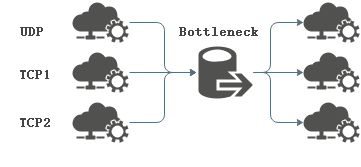
\includegraphics[scale=0.8]{picture/topology1.png}
	\caption{网络拓扑图}
	\label{fig:topology1}
\end{figure}

\subsubsection{丢弃概率}
随机早期检测最难把握的地方就在丢弃概率的选择,因为$P$不是一个常数,而应该随着网络状况和硬件条件改变,初始的分组标记概率P是平均队列长度的线性函数:
\begin{equation*}
	P=max_p(avg-min_{th})/(max_{th}-min_{th})
\end{equation*}

参数$max_p$是标记概率的最大值,当达到平均队列的长度上限时取到。

\begin{figure}[H]
	\centering
	\includegraphics[scale=0.6]{picture/p.png}
	\caption{丢弃概率对吞吐量的影响}
	\label{fig:p}
\end{figure}

在仿真测试中,我们选取了从0到1间距0.1的11个值,同时构建了一张网络拓扑图:瓶颈节点将接受来自三个节点的UDP和TCP混合流量,再将这些混合流量转发给各种的接收方,可以看到由于UDP的无连接性,它几乎不受到丢弃概率的影响始终维持较高的吞吐量,而TCP1和TCP2由于其面向连接的特性,吞吐量非常小,但同时也很明显地看出,TCP流量并没有随着丢弃概率的增加或者减小有正负相关性,反而出现在一定概率左右稳定,超出后大量衰减或增加的现象。

\subsubsection{平均队列权值}

随机早期检测中$W_q$影响平均队列长度,当$W_q$取值较大时,平均队列长度容易受到瞬时性改变,平均队列长度将在短时间内剧增;当$W_q$取值较小,平均队列变化不大,对可能到达的拥塞不敏感,这样调节效果不佳。平均队列长度由以下迭代式给出:

\begin{equation*}
	avg^{n+1}=(1-W_q)avg^{n}+w_q*Qlen
\end{equation*}

由此可见,参数avg是由当前队列长度和旧平均队列长度综合权值得来。

\begin{figure}[H]
	\centering
	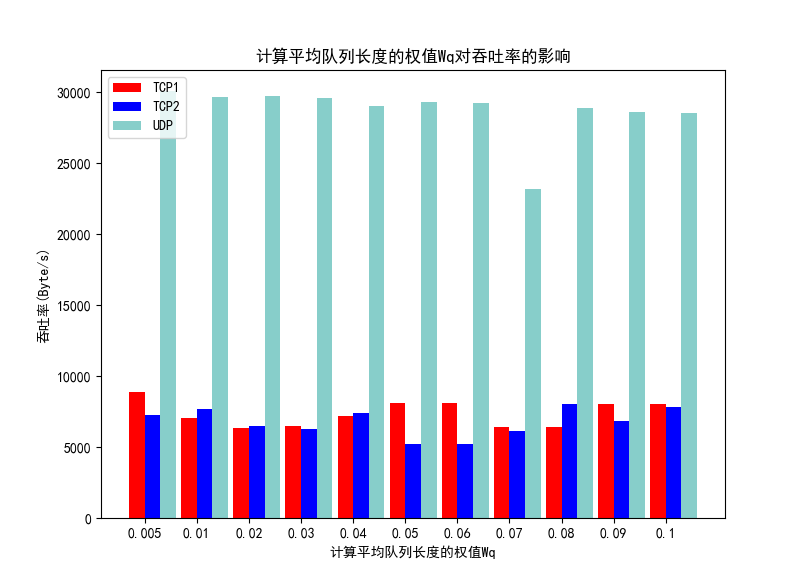
\includegraphics[scale=0.6]{picture/Wq.png}
	\caption{平均队列长度的权值对吞吐量的影响}
	\label{fig:Wq}
\end{figure}

我们仍旧使用以上拓扑结构进行仿真实验,这次UDP流量仍然超出TCP1和TCP2很多,但其中明显受到平均队列长度的影响,在$W_q=0.07$时有较大衰减;与此同时,TCP流量都呈现出两边较高中间较低(抛去0.05-0.06),这说明仅仅从理论上分析出$W_q$不能极端取值,也不意味着维持中立就能获得较好的吞吐量,甚至极有可能比一般情况更差。

\subsection{TCP拥塞控制}

TCP拥塞控制的目标在于最大化利用网络上瓶颈链路(Bottleneck)的带宽,直至瓶颈链路因为过多的流量而产生错误(丢包、不可达),一旦出现这种错误TCP就通过动态化调整自身发送字节的速率来保证接下来传输速率的恢复。

不同的拥塞控制算法思想由于其切入点有差异,可能会带来完全不同的效果,因此本次实验试图模拟在某一特定环境下不同拥塞算法的性能差异。

\subsubsection{拥塞模拟概述}

整个实验过程基于两个点对点相连的路由,拥塞算法则选择了$Vegas$,$Veno$,$WestWood$,,路由分别采用$DropTail$主动队列管理算法,同时在接受路由上加入了错误因子使得报文有一定概率在数据链路层就被丢弃,这会导致接收端无法收到想要的回送报文,继而让发送端产生网络拥塞的错误判断后启动拥塞算法。以下是三种拥塞算法的介绍:

\begin{itemize}
	\setlength{\itemsep}{0pt}
	\setlength{\parsep}{0pt}
	\setlength{\parskip}{0pt}
	\item [1)]Vega不通过丢包来检测拥塞现象,而是通过吞吐量来预测进而动态变化调整窗口,它定义两个常量$a,b(a<b)$,当$Diff< a$时,则线性增加拥塞窗口;当$Diff> b$时,线性减少拥塞窗口。这种拥塞控制方式是在拥塞将要发生时控制,而不是在拥塞发生后控制。
	\item [2)]Veno是对Reno算法中的慢启动(Slow Start)、拥塞避免(Congestion Avoid)、快速重传(Fast Retransmit)和快速恢复(Fast Recovery)等机制进行进一步改进。在拥塞避免阶段,它调整了窗口大小的衰减速率,使其能够更长时间处于较大的窗口而不至于迅速减小。在快速重传阶段,Veno适当降低了慢启动门限值(ssthresh),使TCP窗口大小处于较大值状态。
	\item [3)]WestWood同样在Reno基础上增强了窗口控制和退避处理,当接受到ACK报文时,将此报文的大小除以经过的时间,得到当前带宽的一个评估值。当WestWood在调整窗口时候,重新调整到可用带宽处,而不是简单地将窗口减半。
\end{itemize}

\subsubsection{实验结果与分析}

\begin{figure}[H]
	\centering
	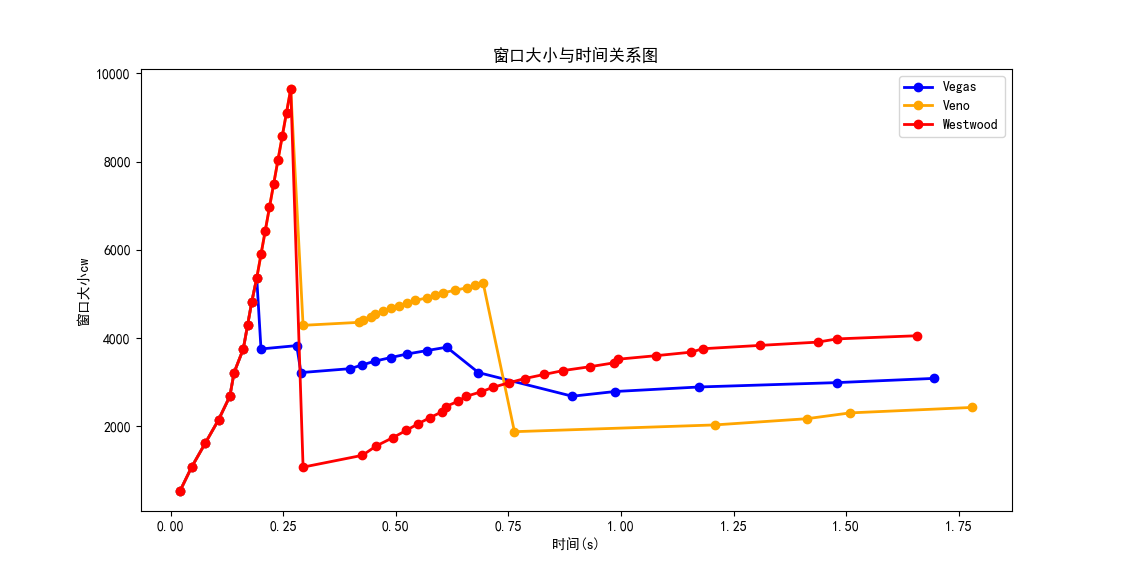
\includegraphics[scale=0.6]{picture/cwTcp.png}
	\caption{TCP窗口大小与时间关系}
	\label{fig:cWTCP}
\end{figure}

在0.25s时发生了一次丢包事件,这可能是路由的队列管理或者校验和错误,Venos、WestWood都有非常明显的下降趋势,WestWood的下降比率达到了将近$90\%$,而Veno也有$50\%$左右,相比之下Vegas则由于其较小的增速与减速率维持住了一个较好的平衡。

在0.75s时由于错误因子的偶发性导致Vegas和Veno都遭遇了丢包,WestWood窗口大小超越了前两者并持续到了实验结束,但三种算法的窗口大小都已接近于收敛,彼此差距都很小。

\begin{figure}[H]
	\centering
	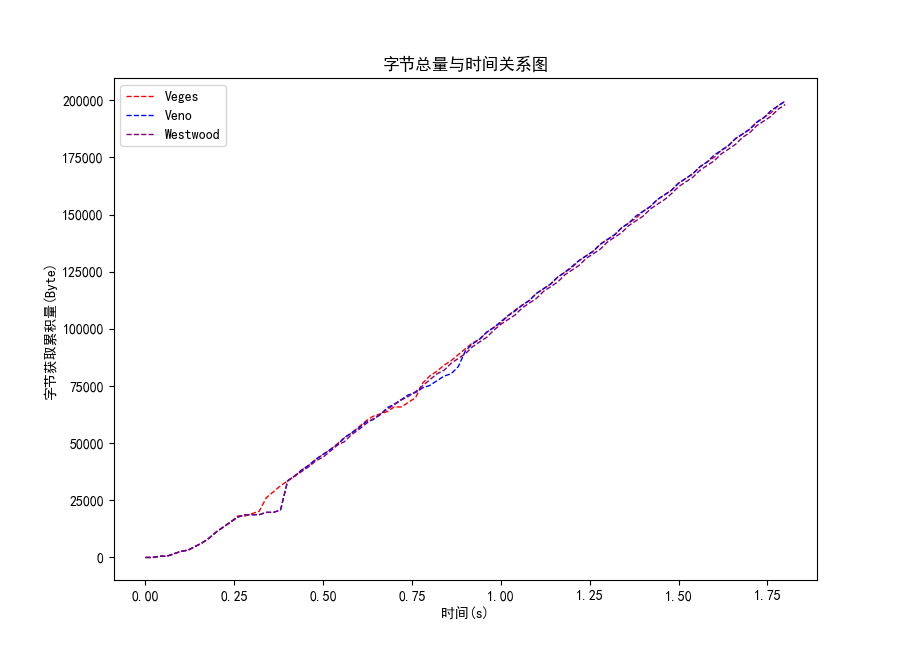
\includegraphics[scale=0.5]{picture/byteTcp.png}
	\caption{字节总量与时间关系图}
	\label{fig:byteTCP}
\end{figure}

虽然在窗口大小上每种算法都经历了各种窗口大小的变化,但是从宏观角度,接收方所得到字节总量并没有发生太大区别,其主要原因有:(1)错误因子设置的比较小这也符合标准情况下网络链路出错概率较小的情况;(2)网络速率较快,短时间内的丢包将迅速被重传机制,快恢复机制所改正。

经过以上实验,我们可以看到在标准环境下,WestWood凭借其算法特性窗口大小浮动很大,而Vegas和Veno则相对稳健,其中Veno更是能够在丢包事件中实现接受字节数小幅度减少。

\section{CSMA/CA实验}
\subsection{802.11Mac层协议}

CSMA/CD要求一个站点在发送数据的同时不断检测信道,而一旦发生碰撞,则停止发送。在无线领域由于无线信号的传输条件十分特殊,信号强度的动态范围非常大,所以在无线适配器上收到的传输信号往往远小于发送的信号强度,因而802.11适配器无法实现碰撞检测。

同时,由于无线电波向所有方向传播但传播距离有限的特性,我们可以将模型抽象为作用范围为一个圆形,同时存在遇到障碍物的隐蔽站问题。所谓隐蔽站,就是同时想和两个站通信的两个站点之间由于距离比较远,彼此检测不到各自发出的信号,所以各自在检测到信道空闲的时候向同一个站点发送数据,结果导致了碰撞,而且检测不到,这就是隐蔽站问题。

因此,在802.11委员会指定无线局域网的协议的时候,必须考虑以下几条问题

\begin{enumerate}
	
	\item {适配器无法实现碰撞检测}
	\item {检测信道空闲问题}
	\item {解决隐蔽站问题}
	
\end{enumerate}

802.11协议组于1997年提出了802.11的物理层和MAC层的协议规范,大大推动了无线局域网的应用和发展。也就是使用CSMA/CA协议,CA是碰撞避免的意思,表明了设计的初衷是为了尽量减少碰撞发生的概率。

值得注意的是,802.11标准设计了独特的MAC层,这是通过协调功能来确定在基本服务集上的移动站,在什么时候能发送数据或者接受数据。协议所定义的 MAC 层的协议中主要有 DCF(分布式协调功能)和PCF点协调功能)协议。DCF是基于CSMA/CA的随机竞争接入方式,而PCF是集中式接入方式,主要应用在基础架构网中。由于 PCF 是可选机制,而且在实际应用中较少采用,所以本文主要讨论的是DCF的性能分析。

分布协调功能DCF不采用任何中心控制,而是在每一个节点使用CSMA机制运行分布式接入算法,通过每个站点的争用来获取信息的发送权,也就是DCF向上提供争用服务。协议规定,所有站点实现必须有DCF功能。为此,802.11协议提出了两个重要时间间隔,即段帧间间隔SIFS和分布协调功能帧间间隔DIFS。

在争用的过程中有几个重要参数。由于发生冲突而进入推迟接入状态的各个站点必须同时在争用期执行统一的算法公平的争用信道,因此争用期也就是争用窗口CW的概念尤为重要。退避算法规定在进入争用期的时候,在0到CW的间隙中随机生成一个退避时隙数,并且设置退避计时器,而在几个站点争用的时候计时器最先降为零的站点将首先接入,而同时冻结其他计时器,在下个争用信道时才接着倒计时。因此这样的算法对所有站站点而言是公平的。

802.11建议争用窗口的最小值取为15,最大值为1023。后面将会对CW的不同设定进行分析。

同时在无线局域网中有一个重要参数距离中心点的距离。由于信号传播的特殊性,信噪比较低,导致在较远的距离时信号衰减已经比较严重,本文同时对参数距离进行了分析。

\subsection{DCF原理}
DCF是802.11中定义的MAC协议,主要针对于竞争模式,这是一种异步数据传输方式,主要应用在自组织网络中。该协议以CSMA/CA为基准,采用冲突避免的策略来降低网络中的数据冲突率。

自组网络,也就是没有固定基础设施的无线局域网,这种自组网络没有集中的接入点AP,局域网中各个站点处于平等状态,而为了研究的一般性,本文依然采用具有接入点AP的无线局域网络。

DCF的基本原理是:节点在发送数据前首先侦听信道,如果信道空闲且时间超过DIFS,则节点发送数据帧;如果检测到信道忙,则生成一个随机的退避时间,启动退避计数器,一直等到信道空闲且空闲时间超过DIFS,退避时钟计数器按时隙为单位减少;信道忙时则暂停,直到信道重新空闲且空闲时间超过DIFS后才恢复计时。当退避时钟计数器减为零后,如果信道空闲时间超过DIFS,节点则发送数据帧,否则重新启动退避计数器。当节点发送数据失败后,竞争窗口值加倍。而在五次重传后设定不再加倍,这受到最大争用窗口的限制。

DCF有两种模式:一是基本接入模式Basic,即当侦听信道空闲且空闲时间超过DIFS后,直接发送数据,等待对方发送ACK信号,以便发送下一帧,具体传输时间可以表示为

\begin{equation}
T_{bas} = DIFS + DATA + SIFS + ACK
\end{equation}

二是RTS/CTS模式,即当侦听信道空闲且空闲时间超过DIFS后,不直接发送数据,而先发送一个很短的RTS控制帧来预留信道,接收方通过向发送方反馈CTS帧确认收到正确信息。发送方收到CTS帧后才开始发送数据帧,等待对方发送ACK信号,以便发送下一帧。由于在RTS/CTS模式下只有RTS帧会发生碰撞,通常情况下,RTS控制帧都比较短,协议一般设定RTS帧长为20个字节,CTS帧长为14个字节,所以能有效地减少碰撞时间,提高系统的性能,具体发送时间可以表示为

\begin{equation}
T_{rts/cts} = DIFS + RTS + SIFS + CTS + SIFS + DATA + SIFS + ACK
\end{equation}

本段将对基本模式和开启RTS/CTS的模式进行网络性能比较,衡量参数主要是网络整体的吞吐量和传输延迟,具体对比环境为低速网络和高速网络,数据长度较长和较短这两大类不同方式下传输的性能。

本节中的推导都基于以下的假设:信道为理想信道,可知冲突是数据传输失败的惟一原因;系统始终处于饱和状态即每个站点要发送数据队列始终不为空;发送的数据包发生碰撞的概率恒定且相互独立;重传次数没有限制,直到重传成功。
\subsection{DCF性能分析}

首先是DCF设计的一般参数实验,DCF的主要参数有

\begin{itemize}
	\item {工作站点数量}
	\item {数据传输率}
	\item {争用窗口大小}
	\item {接入点和工作站时间的距离}
\end{itemize}

为控制变量,在此处设置RTS/CTS均为关闭的状态。

在使用NS3仿真的初始设定中,设置的参数如下,工作站点数量:1个,工作站距离AP的距离为25m,数据包大小默认设置为2000字节,最小争用窗口15,最大争用窗口1023。以上参数设定在进行仿真的时候都可以通过输入参数修改,而基本上对每一个参数的研究都需要设定大部分参数,所以将这些默认参数设定为协议建议的或是比较通用的,对后续仿真也较为适用。

本文首先从工作站数量开始,我们选取了从较少的5个工作站到较多的40个工作站同时在一个BSS中传输信息,观察系统吞吐量。在图\ref{fig:contention}中,可以看到在默认传输速率下,在不同工作模式下,工作站数量增多均会导致整体性能的下降,在基本模式中虽然工作站数量较少的情况下总吞吐量很高,但是随着数量增加,信号碰撞增多,竞争不断增多,导致系统性能急剧下降。而在开启RTS/CTS的情况下,可以看到虽然在初始点的吞吐量受到传输两类控制帧的限制,并不算很高,但是在数量增加到一定程度也并没有太大波动,而是在小范围内小幅减小,可以说整体性能影响并不大。
\begin{figure}[ht]
	\centering
	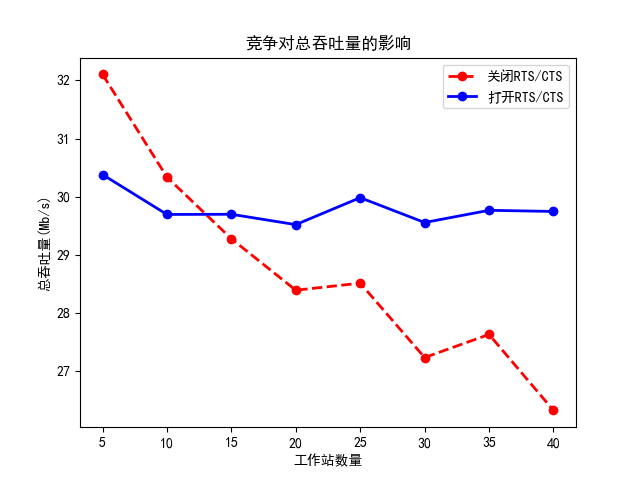
\includegraphics[scale=0.6]{picture/contention.png}
	\caption{接入站竞争对网络性能的影响}
	\label{fig:contention}
\end{figure}

接下来控制接入点数量为20个,在这种情况下我们选取不同的争用窗口cwMin和cwMax,来分析对性能的影响。首先是最小争用窗口的设置,这里控制最大争用窗口为1023个时隙。本文选取了几个重要的大小进行仿真,可以看到如果最小值选的过小,整体性能并不算很好,而建议设定的参数15在仿真过程中也没有得出最佳的性能,整体较好的性能出现在150到200之间。在图\ref{fig:cwMin_Max}中对cwMin看的不是很清楚,这里放出原始数据表\ref{tab:cwMin}。

\begin{table}[]
	\centering
	\begin{tabular}{llllllll}
		\hline
		cwMin      & 3       & 15      & 50      & 100     & 250     & 500     & 1000   \\
		\hline
		Throughput & 26.0543 & 28.3936 & 30.8834 & 31.8698 & 31.4822 & 28.9347 & 24.434 \\
		\hline
	\end{tabular}
	\caption{不同cwMin对总吞吐量的影响}
	\label{tab:cwMin}
\end{table}

可以看到系统的最佳部分出现在cwMin为100左右。在大于100的情况下网络性能便急剧下降,且总吞吐量和最小争用窗口有线性减少的关系。

\begin{figure}[ht]
	\centering
	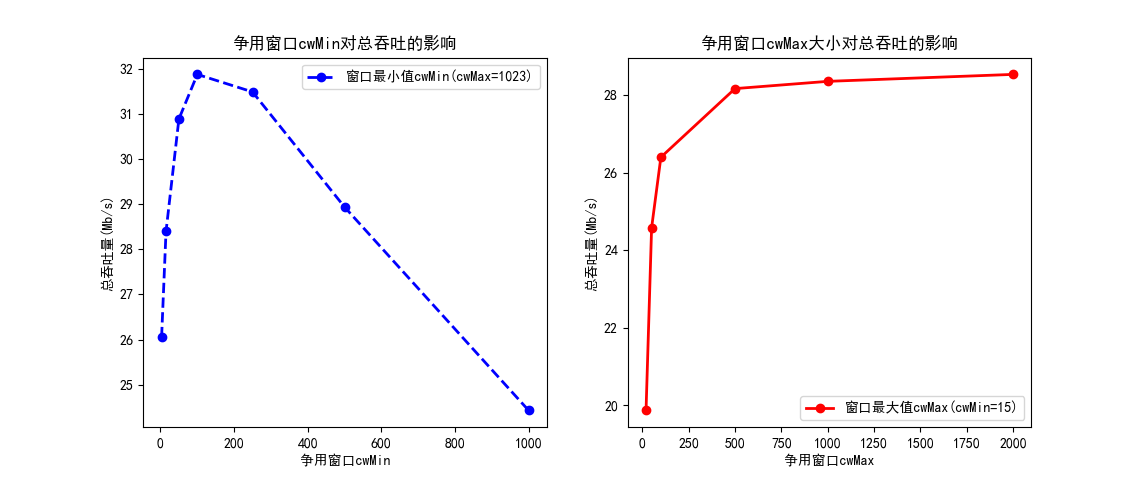
\includegraphics[scale=0.6]{picture/cwMin_Max.png}
	\caption{争用窗口对总吞吐量的影响}
	\label{fig:cwMin_Max}
\end{figure}

在分析最大争用窗口的时候,本文设定最小窗口为协议建议的15个时隙,而不是实验发现的最好的最小窗口。依赖这是出现在最大窗口固定为1023的情况下,而来没有细致选取区间进一步分析,没有寻找到cwMin和cwMax两个参数时间的联系,所以也就选取最小窗口为15。实验发现,最大窗口值在500之前,会导致总吞吐量的急剧增加,而在之后增加的窗口值影响并不太大,在802.11b协议中超过1023的设定更是没有影响,这是因为受到协议的制约。

协议CSMA/CA规定,为了减少碰撞的机会,不管是发生碰撞还是数据帧传输出现了差错,也就是没有受到确认帧的情况下必须重传,每重传一次使得争用窗口的数值近似加倍增大。

常用退避算法有三种:非坚持,1-坚持,p 坚持。非坚持算法采用随机的重发延迟时间可以减少冲突发生的可能性,可是这样处理会降低媒介利用率,1-坚持型算法虽然能够避免了媒介利用率的损失,但是假如有两个或两个以上的站点有数据发送,冲突就不可避免。 而p坚持既能像非坚持算法那样减少冲突,又能像 1-坚持算法那样减少媒介空闲时间的,然而p值较难选择,最终实现比较困难,由于无线通信的特性,802.11协议选择的是非坚持退避算法,减少冲突发生的可能性,也既是CSMA/CA 的目标所在。

由于协议设定当出现5次或者5次以上的重传时,随机退避的时隙应该在0到1023之间生成,争用窗口cw就不再增大了。所以超过1023的cwMax设定对整体影响不大。

\begin{figure}[ht]
	\centering
	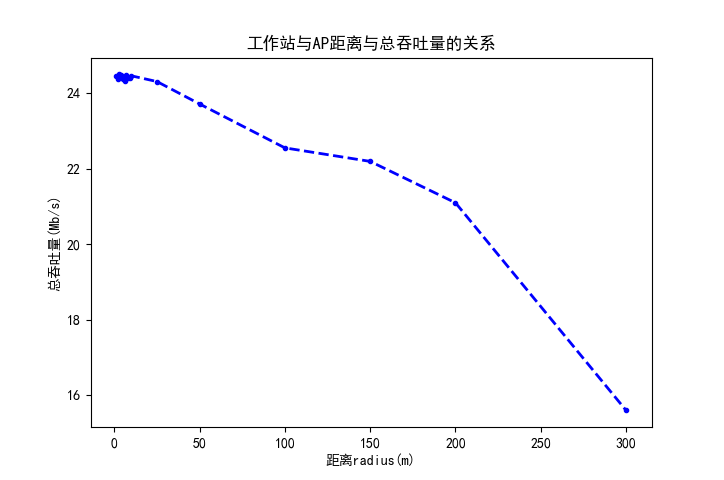
\includegraphics[scale=0.6]{picture/radius.png}
	\caption{站点距AP长度对总吞吐量的影响}
	\label{fig:radius}
\end{figure}

本文就工作站距离AP的距离进一步分析。一开始选取距离间隔较大,范围较广,从10m到300米的范围。而实际情况中无线局域网的有效范围一般不会超过150m,此处选定到300m是考虑到理想情况下的参数设定,结果也表明在较远距离下确实能够传输,但是性能急剧下降。从图\ref{fig:radius}中可以看出在较近的距离下传输性能较好,而随着距离的增加大致上呈现三个趋势,一是从0到100m的过程,此时吞吐量下降较为缓和,但也是呈现一个近似线性的曲线;第二阶段是100m到200m,此时性能趋于平稳,分析认为这是无线局域网的边界传输范围,在这个范围内传输的性能影响不会很大;第三阶段是大于200m的过程,此时已经超过边界范围,因此性能急剧下降。

可以看到在较近的区间内点的分布比较密集,这是由于在第一次实验后发现整体曲线较为平滑,因而进一步探寻在较近的情况下是否会出现较大波动的情况,所以设置了0到20的仿真。结果表明在这个范围内整体吞吐量并没有较大变化,所以在图中呈现出密集的情况。
\subsection{RTS/CTS对传输性能的影响}

对于RTS/CTS的性能分析,主要从两个方面进行。高速传输信道和低速传输信道的对比以及较短帧长和较长帧长在两个模式下的不同表现。

首先是较短帧长的分析,在图\ref{fig:RTS_CTS_shortpacketLen}中,实现设置了不同速率下,两种模式的性能表现对比。可以看到在低速链路中,传输速率为5Mbps的情况下,较少的竞争对网络性能影响不大,而当工作点超过5个的时候基本模式的性能要相对优于开启RTS/CTS的模式,也就是说在基本模式中吞吐量的增长区间要比开启RTS/CTS的模式长,这导致了后续冲突发生时,基本模式吞吐量较高。

在高速链路中,可以看到基本模式的性能远远优于开启RTS/CTS的模式,并且随着节点数量增加,都有不同程度的下降,区域平稳,但是基本模式受到影响较大,RTS/CTS模式受到影响较小。

\begin{figure}[ht]
	\centering
	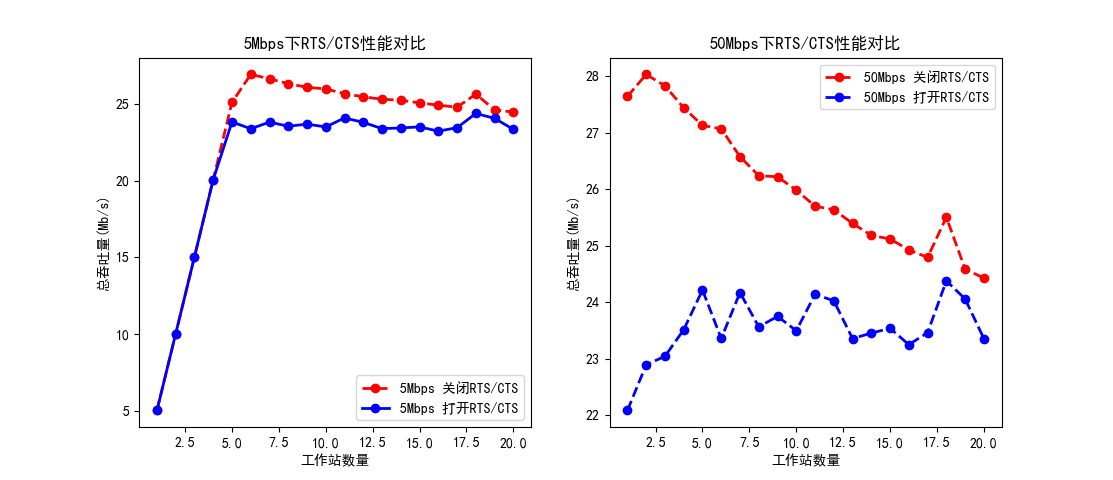
\includegraphics[scale=0.6]{picture/RTS_CTS_shortpacketLen.png}
	\caption{短帧长下两种模式的对比}
	\label{fig:RTS_CTS_shortpacketLen}
\end{figure}

观察分析图\ref{fig:RTS_CTS_longpacketLen},对于传输长帧长的情况又有不同,此时在低速链路中,在工作点较多的情况下RTS/CTS模式发挥了作用,在工作站约为12个的时候RTS/CTS模式超过了基本模式,在高速链路的情况下,尽管站点数量较少的情况下基本模式性能极佳,而一旦冲突增多,吞吐量也急剧下降,而RTS/CTS模式此时发挥作用,让整个网络性能保持在较好的状态。

\begin{figure}[ht]
	\centering
	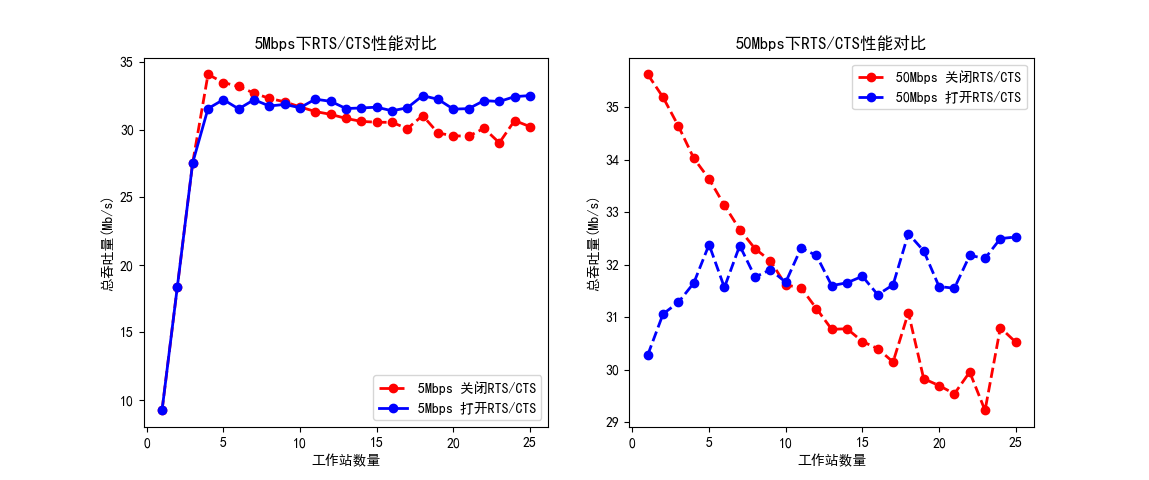
\includegraphics[scale=0.6]{picture/RTS_CTS_longpacketLen.png}
	\caption{长帧长下两种模式的对比}
	\label{fig:RTS_CTS_longpacketLen}
\end{figure}

因而由仿真结果分析可知,在传输较短的数据帧情况下,高速链路中使用基本模式优于RTS/CTS模式,低速链路性能差别不大;在传输较长的数据帧的情况下,高速链路中RTS/CTS的优越性发挥出来,低速链路同样RTS/CTS的性能占优。这和我们熟知的较长帧适用RTS/CTS模式,较短帧适用基本模式的知识一致,然而链路在高速链路适用RTS/CTS模式,中低速链路中适用基本模式这样的结论\cite{1}没有很好证明。因此分析认为在传输过程的两对矛盾中,高速传输信道和低速传输信道的对比以及较短帧长和较长帧长的对比中,数据帧长是主要矛盾,链路传输速率是次要矛盾,RTS/CTS模式的选择与否主要取决于传输数据帧的长度。

\subsection{传输延迟}
前文主要讨论了DCF参数对于网络总体吞吐量的影响,现在简单讨论对于延迟的影响。为使得模型简化,本文没有模拟真实的网络,而是模拟在理想信道中传输的效果。因此忽略了信道质量对性能的印象,造成延迟的原因只能是发生冲突导致的。

我们定义单个节点的平均延迟是指发生退避开始到帧完成传输的平均时间间隔,$\tau$为节点在随机选择时隙的时候选择发送的概率,$n$为网络节点数量,$p$为除去正在发送信息的节点的剩余$n-1$个节点至少有一个发送数据包的概率,则$p=1-(1-\tau )^{n-1}$,那么在其余$n-1$个节点中两个连续忙的时隙之间的空闲时隙的平均个数为$n_{it}=\sum_{i=0}^{\infty}{i(1-p)^{i}p}=\frac{1}{p}-1$。

同时,我们定义$p_{1send}$为在$n-1$个节点中至少有一个发送的前提下,只有一个点发送的概率,用条件概率的表达式可得
\begin{equation}
p_{1send}=\frac{(n-1)\tau(1-\tau)^{n-2}}{p}
\end{equation}

在对DCF原理的分析中已经分析发送一个帧所需要的时间,现在具体将时间拆分为成功传输数据使得信道忙碌的平均时间$T_{s}$和节点之间产生碰撞而使得信道忙碌的平均时间$T_{c}$,那么可以得出在一个点发送信号的情况下,其余$n-1$个点在连续两次传输过程中的平均时间间隔
\begin{equation}
T_{rc}=p_{1send}T_{s}+(1-p_{1send})T_{c}+n_{it}\sigma
\end{equation}
我们称之为更新周期。其中$\sigma$表示为每一个时隙的具体长度。

同时,我们总结退避时间的函数表达式为
\begin{equation}
W_{i}=
\left\{
\begin{aligned}
&2^iW_{0}\quad 
0\leqslant &i\leqslant m-1\\
&2^mW_{0}\quad 			  &i\geqslant m\\
\end{aligned}
\right.
\end{equation}
表示在每一个退避阶段$i$,退避的时间平均值为$(W_{i}-1)/2$,而$W_{i}$表示在退避阶段$i$的窗口大小,$W_{0}$表示设定的初始退避时间。

所以,综上所述节点在退避阶段i要经过$1/2(W_{i}-1)/(n_{it}+1)=(W_{i}-1)p/2$个更新周期,所以节点接连两次重传的平均时间为$(W_{i}-1)pT_{rc}/2$,那么节点在退避阶段i成功发送数据所经过的延迟$T_{d}^{i}$可以整理为
\begin{equation}
T_{d}^{i}=\sum_{i=0}^{\infty}(W_{k}-1)pT_{rc}/2+(i-1)T_{c}+T_{s}
\end{equation}
所以平均延迟可以表示为
\begin{equation}
T_{d}=\sum_{i=0}^{\infty}(1-p)p^{i-1}T_{d}^{i}
\end{equation}

\begin{figure}[ht]
	\centering
	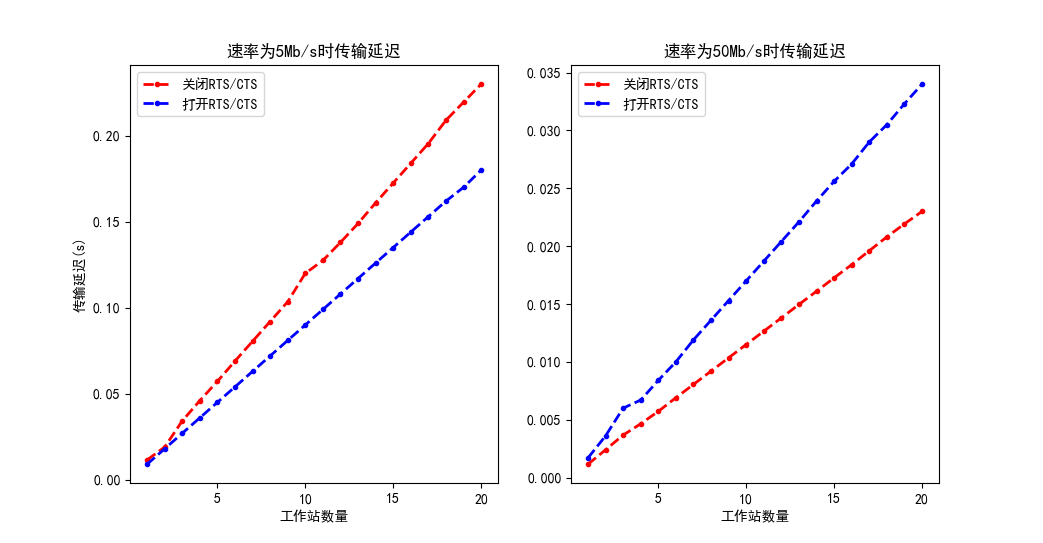
\includegraphics[scale=0.6]{picture/delay.png}
	\caption{低速率和高速率下两种不同模式的传输延迟}
	\label{fig:delay}
\end{figure}
通过构建模型,使用NS3仿真,得出了在低速率和高速率下两种不同模式的传输延迟的对比,具体如图\ref{fig:delay}。可以看到,在低速率信道下使用基本模式延迟较高,使用RTS/CTS传输延迟较低。而在信道处于高速率的情况下使用基本模式传输延迟又比较小,使用RTS/CTS模式对传输延迟的影响比较大。虽然在拟合曲线的过程中存在一些特殊数据的点,但是总体上传输延迟和工作站数量呈现一个线性关系,曲线的倾斜程度可以理解为网络系统对工作站数量响应的敏感程度。

在低速和高速信道的情况下,传输延迟都和工作站数量呈现线性关系,而低速率下由于碰撞造成的时间损失较大,所以采用RTS/CTS模式能减少冲突,从而降低传输延迟,而仅仅是多花费了传输少量RTS/CTS的时间。而在高速率信道中,如果发生冲突,也能较快退避并等待恢复,对网络整体性能影响较小,所以此时基本模式传输延迟较低,性能较好。
\subsection{分析}

由仿真验证可知,RTS/CTS模式下DCF在低速数据传输中吞吐量性能比基本接入模式下好,尤其是在节点数增多的情况下。在高速传输时情况恰恰相反,基本接入模式的性能比较好。从总体上看,延迟与站点数的多少基本上成线性增长关系。

造成这种现象的主要原因是由于基本接入方式和RTS/CTS方式的本身机理不同,由于RTS/CTS多了RTS帧和CTS帧交互的一个过程,一方面就是通过RTS帧和CTS帧的交互,能够预先预留信道,这样能有效地降低碰撞概率和碰撞时间,这就是为什么在低速的情况下RTS/CTS的性能普遍优于基本方式的原因,低速情况下通过提前预约信道,减少了冲突,从而提高传输性能,但是较高链路由于传输较快,就算发生了冲突也能很快调整并退避,此时RTS/CTS方式反而成了负担。

但是另一方面由于RTS/CTS方式将大量的时间都消耗在RTS帧和CTS帧的交互上了,真正传输数据的时间并不是很长。这也在理论上解释了在较短帧长的情况下使用RTS/CTS方式会导致吞吐率的下降,也就是一个传输时间单元中传输有效数据的时长较短,有效吞吐率较低,而在较长帧长的情况下使用RTS/CTS方式能有效提高整体性能吞吐率,此时避免冲突的效果比较好。

\section{5G的非组网架构双连接仿真实验}
\subsection{5G多连接的必要性}
毫米波(mmWave)频段--指的是一种特殊电磁波,波长为1毫米到10毫米,波动频率为30GHz-300GHz。相对于6GHz以下的频段,毫米波具有大带宽、低空口时延和灵活弹性空口配置等独特优势,可满足未来无线通信对系统容量、传输速率和差异化应用等方面的需求。然而,使用毫米波频段提供稳定服务仍需要克服一个关键性障碍,信道间歇性。毫米波信号会被许多常见的建筑材料所阻挡,比如砖头和玻璃。甚至人体也会造成高达35dB的的衰减。因此,由于客户端UE在不同Cell间的移动,障碍相对UE的移动、甚至手机在手上的微小移动,都可能导致信道迅速出现或消失。多连接是提高毫米波系统稳定性的主要工具之一。即每个移动设备UE或用户设备保持与多个Cell的连接。这里的多个Cell可能包括5G毫米波Cell和/或传统4GLTE Cell。在一条链路被阻断的情况下,UE可以找到替代的路线来保持连接。
\begin{figure}[ht]
	\centering
	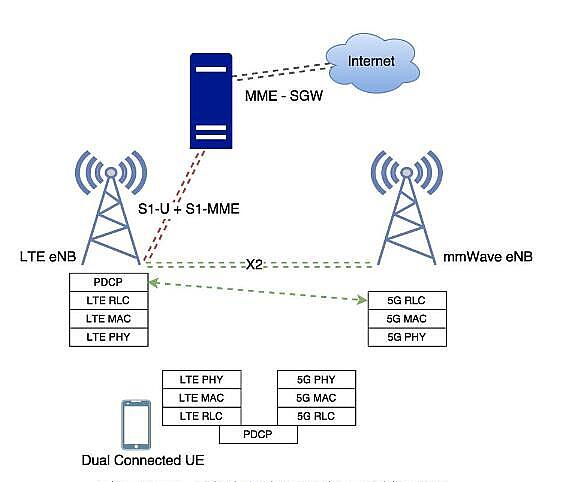
\includegraphics[scale=0.6]{picture/5G-SNA.jpg}
	\caption{LTE-5G tight-integration architecture}
	\label{fig:delay}
\end{figure}
\subsection{双连接(DC)的原理}
使用双连接(DC)是一个不同的和更强大的解决方案,UE同时连接到LTE和毫米波BS。LTE Cell作为一个备份:由于UE已经连接,当mmWave链路的信号质量下降时,不需要用随机接入程序进行完整的切换,也不需要向核心网发送路径切换消息。从LTE BS到UE的单一RRC控制消息就足够了。LTE Cell也是所有邻近mmWave Cell的协调者,并且是双连接设备进入核心网络的接入点。在这种设置中,UE发射试点,mmWave基站可用于估计链路质量(例如通过测量SNR)。这些测量值通过X2接口定期从每个mmWaveCell发送到LTECell。因此,LTE BS知道哪个是每个UE的最佳mmWave Cell。
\subsection{ns-3 mmWave模块仿真实验}
借助ns-3 mmWave McUeNetDevice,可以模拟类似于图 11中的场景:在其覆盖范围下有一个 LTE eNB 和多个毫米波 eNB,要么位于同一位置,要么通过 X2 接口连接。根据 ns–3 中可用的移动模型,UE 可以以不同的速度移动,而在移动时,根据其位置和与 eNB 的距离,UE 会遍历不同的信道条件。这些方案可用于评估不同移动性管理和多连接方案的性能。
\begin{figure}[ht]
	\centering
	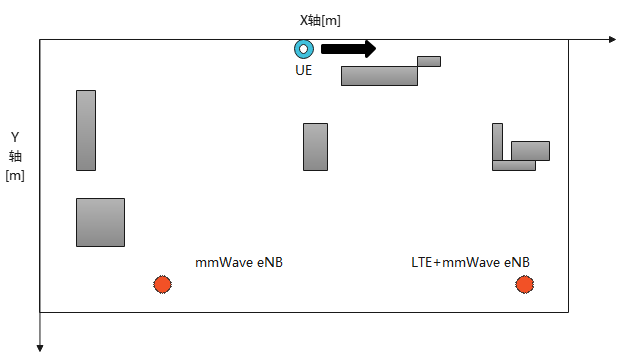
\includegraphics[scale=0.6]{picture/buildings.png}
	\caption{模拟场景}
	\label{fig:delay}
\end{figure}

此仿真实验的目的是比较双连接(DC)系统和硬切换(Hard Handover)系统的吞吐量、延迟。当UE 遇到连接中断时,DC架构的好处是显而易见的:由于双连接,它可以立即使用 LTE 链路恢复通信。而独立 UE 必须感知链路故障,然后执行要用随机接入程序进行完整的切换。这需要更多的时间,并导致该时刻吞吐量为零。
\begin{figure}[H]
	\centering
	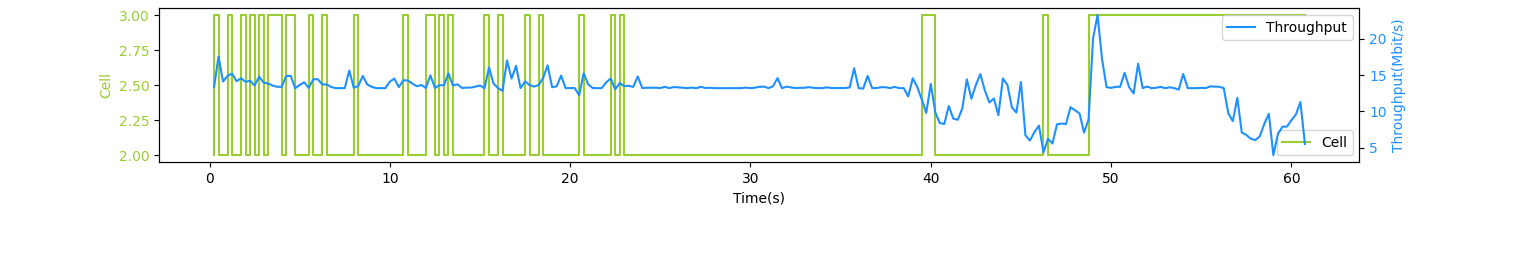
\includegraphics[scale=0.45]{picture/DlRlcStats_Throughput.png}
	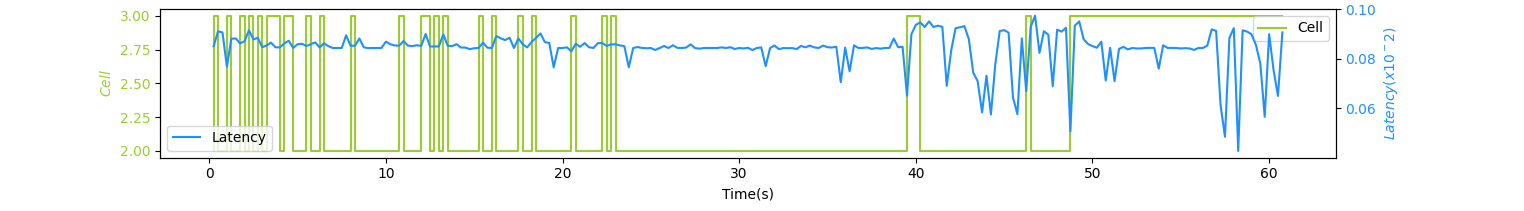
\includegraphics[scale=0.45]{picture/DlRlcStats_Latency.png}
	\caption{双连接}
	\label{fig:delay}
\end{figure}
\begin{figure}[H]
	\centering
	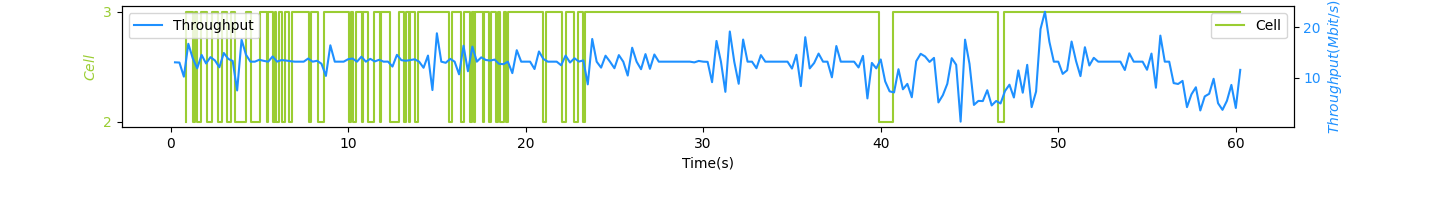
\includegraphics[scale=0.45]{picture/DlPdcpStats_Throughput.png}
	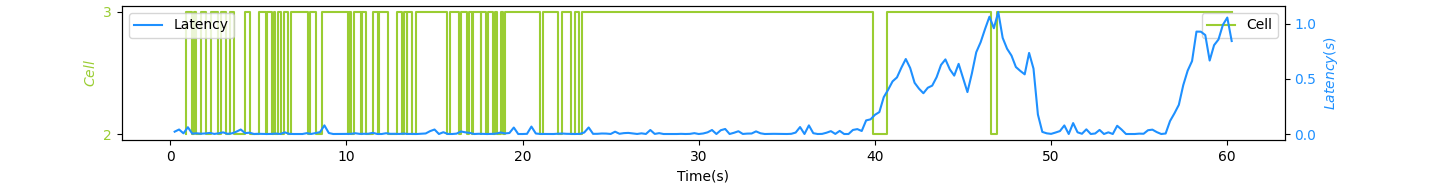
\includegraphics[scale=0.45]{picture/DlPdcpStats_Latency.png}
	\caption{硬切换}
	\label{fig:delay}
\end{figure}

证明了双连通性框架在使用mmWave访问链路的端到端网络的切换管理方面提供了显著的性能改进,包括(i)减少包丢失,(ii)减少控制指令,(iii)减少延迟,(iV)更高的吞吐量稳定性。
\clearpage
\begin{thebibliography}{99}
	\bibitem{1} 白科,胡建平.无线局域网DCF性能分析与仿真[J].现代电子技术,2008(01):13-15+17.
	\bibitem{2} 陈坚刚.IEEE802.11b的DCF退避算法实现技术探究[J].浙江工商职业技术学院学报,2010,9(03):36-39.
	\bibitem{3} M. Polese, M. Giordani, M. Mezzavilla, S. Rangan and M. Zorzi, "Improved handover through dual connectivity in 5G mmWave mobile networks", IEEE J. Sel. Areas Commun., vol. 35, no. 9, pp. 2069-2084, Sep. 2017.
	\bibitem{4} M. Polese, M. Mezzavilla and M. Zorzi, "Performance comparison of dual connectivity and hard handover for LTE-5G tight integration", Proc. 9th EAI Int. Conf. Simulat. Tools Techn. (SIMUTOOLS), pp. 118-123, 2016, [online] Available: http://dl.acm.org/citation.cfm?id=3021426.3021445.
\end{thebibliography}

\appendix
\section{TCP相关}

\subsection {\bf RED代码}
\lstinputlisting[
style       =   Python,
caption     =   {\bf p2.cc},
label       =   {p2.cc}
]{./code/p2.cc}

\section{DCF仿真代码}
\subsection{数据}
\end{document}
